
\subsection{Cross Platform}

Uknow system shall include several clients including: web app, desktop client and mobile app.
The users should have the freedom to choose their preferred platform, and get uniformed user experience.

\begin{figure}[H]
  \centering
  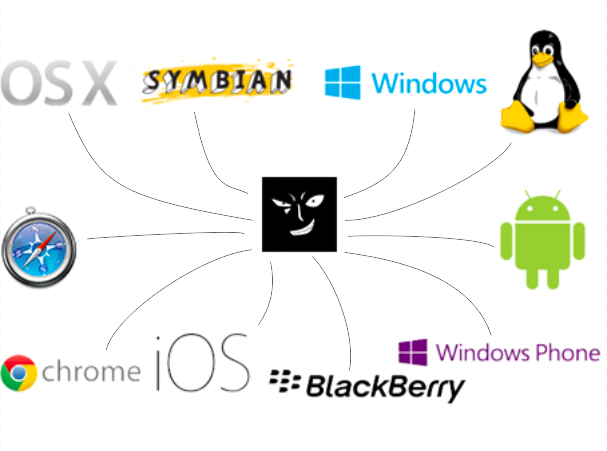
\includegraphics[width=\textwidth]{img/platforms.png}
\end{figure}

\subsubsection{Web app}

Web apps are built in standards-based technologies such as HTML5,
CSS3 and other modern web tech.  Without any special translations,
conversions or re-programming, a web app can run on pretty much any platform with a modern,
standards-compliant web browser. Once a web app is launched, users on iPhones, iPads, Android phones,
the Kindle Fire and Windows Phones can all access the same app and run it just as well as on any other platform.

The web app should render correctly on any of these desktop browsers:

\begin{description}
\item[Google Chrome/Chromium] a freeware web browser developed by Google.
\item[Mozilla Firefox] a free and open source web browser by the Mozilla Foundation and its subsidiary, the Mozilla Corporation.
\item[Safari] developed by Apple Inc.
\item[Opera] developed by Opera Software.
\end{description}

Note that support for Internet Explorer by Microsoft is not planned.

As for mobile browsers, the following platform should be supported:

\begin{description}
\item[Opera Mobile] running in Windows Phone and Symbian.
\item[Safari] pre-installed on all versions of iOS devices.
\item[Chrome Mobile] available in app store for iOS and Android.
\end{description}

\subsubsection{Desktop application}

Considering performance issue that web applications will always run in a sandbox
and won't have full access to native resources and security and interactivity, desktop application
is still needed on many popular platforms including:

\begin{description}
\item[Windows] which dominate the world's personal computer market with over 90\% market share.
\item[Mac OS X] a Unix-based graphical interface operating systems developed, marketed, and sold by Apple Inc.
\item[Linux] a Unix-like and POSIX-compliant computer operating system assembled under the model of free and open source software development and distribution.
\end{description}

For different platforms, different formats of installation file should be provided as:

\begin{description}
\item[Windows] a msi or exe executable file for installation.
\item[Mac OS X] a dmg file containing a standalone app bundle.
\item[Linux] a tarball with a shell script for automatic installation.
\end{description}

\subsubsection{Native Mobile App}

\begin{description}
\item[Android] the app should be available on Google Play Store.
\item[iOS] like Android, user can download the app on App Store.
\end{description}

